\newpage
\section{\emph{SMALL MODULAR REACTORS (SMRs)}} \label{small_modular_reactors}

Los reactores modulares pequeños, más conocidos como \acrfullpl{smr}, son \textbf{reactores nucleares avanzados que producen entre 10 y 300 MWe por módulo} (\cite{nea_smrs_2021}). Aunque se trata de una potencia considerablemente menor a la de los reactores nucleares convencionales de alta potencia ---que suele ser de más de 1.000 MWe---, es precisamente esta característica la que los hace muy atractivos, dadas las múltiples ventajas que esto proporciona en cuanto a versatilidad y variedad de aplicaciones.

Actualmente, hay un creciente interés por esta innovadora tecnología. Durante la \emph{Conferencia Internacional sobre el Cambio Climático y el Papel de la Energía Nuclear} celebrada en septiembre de 2019, muchos Estados Miembros consideraron a los \acrshortpl{smr} como ``una opción nuclear potencialmente viable para contribuir a mitigar el cambio climático'' (\cite{oiea_informe_2019}). A raíz de esta conferencia, en abril de 2021, el \acrfull{oiea} creó la \emph{Plataforma sobre Reactores Modulares Pequeños y sus Aplicaciones (Plataforma SMR)}, un mecanismo que coordina las actividades del \acrshort{oiea} en este campo y proporciona un punto de encuentro común para los Estados Miembros y otras partes interesadas. Por último, cabe destacar que la Comisión Europea creó el pasado 6 de febrero de 2024 una alianza con el objetivo de facilitar y acelerar el desarrollo y el despliegue de los primeros proyectos de \acrshortpl{smr} en Europa a principios de la década de 2030: la \emph{Alianza Europea Industrial en SMRs}. Todo esto refleja una apuesta creciente por los pequeños reactores modulares que debe ir acompañada por un fuerte impulso en el \acrshort{idi} en este ámbito.

\subsection{Breve recorrido histórico: Orígenes y desarrollo}

El origen de los \acrshortpl{smr} es militar y se remonta a los años 50, cuando se diseñaron por primera vez los pequeños reactores que se emplearon para la propulsión naval de submarinos nucleares, portaviones y rompehielos. Con la elaboración del primer subarino nuclear, el \emph{Nautilus}, diseñado por la armada estadounidense y puesto en marcha en enero de 1955, se puso de manifiesto las importantes ventajas que esta tecnología ofrecía a los grandes navíos militares: posibilidad de inmersión por tiempo ilimitado ---en el caso de los submarinos--- al no requerir oxígeno para su funcionamiento, alto nivel de disponibilidad y de independencia de abastecimiento de combustible, elevada versatilidad y mayores velocidades de desplazamiento (\cite{propulsion_naval_nuclear}).

\begin{figure}[h]
    \centering
    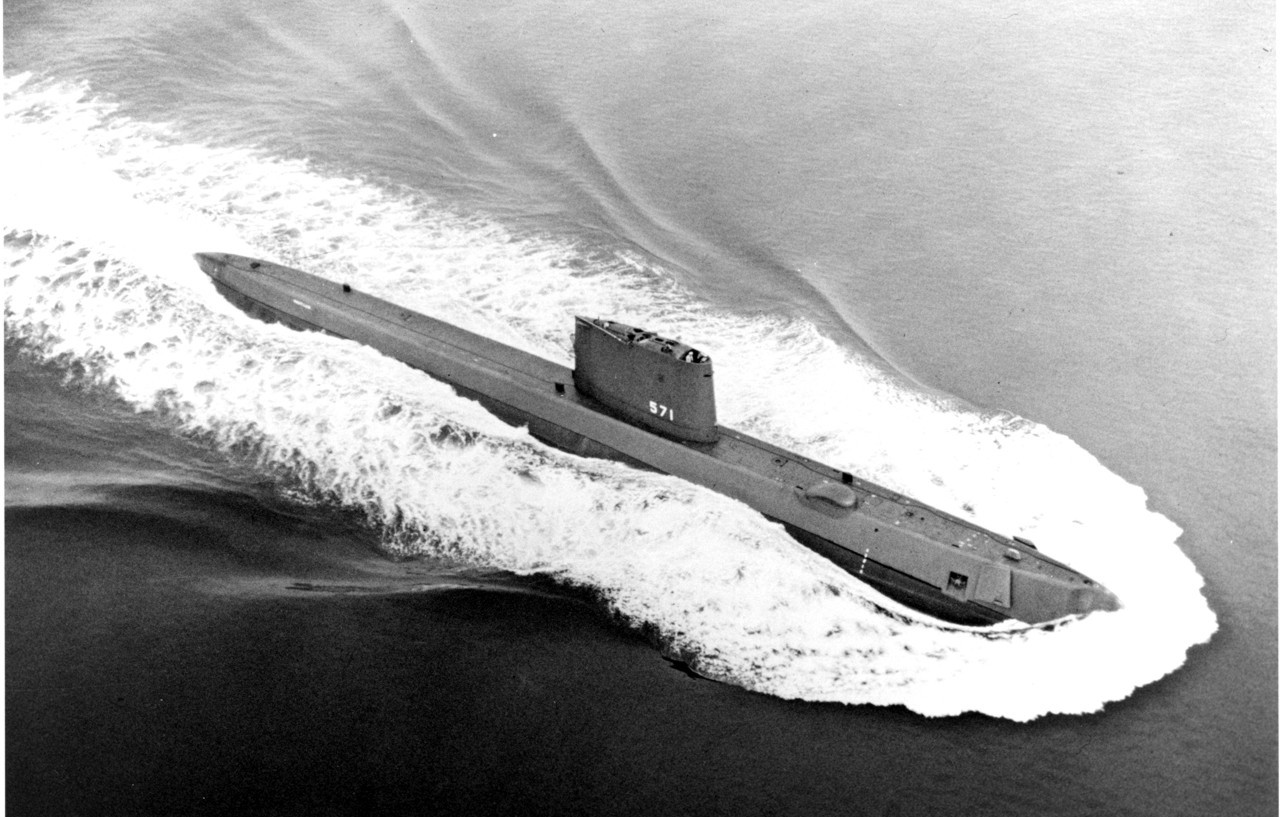
\includegraphics[width=0.55\textwidth]{content/figures/nautilus.jpg}
    \caption{\emph{USS Nautilus (SSN-571)} en alta mar con su reactor S2W de 10 MW de Westinghouse (\cite{poder_naval}).}
    \label{fig:nautilus}
\end{figure}

No fue, sin embargo, hasta más adelante cuando empezaron a desarrollarse los pequeños reactores nucleares comerciales para uso civil. El primer prototipo fue diseñado en 2007 por un equipo de científicos estadounidenses de la \emph{Oregon State University (OSU)} y se le llamó \emph{Multi-Application Small Light Water Reactor (MASLWR)}. Con una potencia de 45 MWe, el MASLWR, fue el prototipo con el que empezó a trabajar la empresa \emph{NuScale Power}, la cual consiguió lanzar en 2022 al mercado estadounidense el primer \acrshort{smr} apto para operar.

Hoy en día \textbf{existen en todo el mundo más de 80 diseños y conceptos de \acrshort{smr}} en diversas etapas de desarrollo, cuatro de los cuales se encuentran en etapas avanzadas de construcción en Argentina, China y Rusia.

\subsection{Clasificación de los Small Modular Reactors}

Pese a que existen diversos criterios para determinar los distintos tipos de \acrshortpl{smr}, en el presente proyecto se ha escogido la clasificación realizada por el \acrshort{oiea}, en la que se distinguen 6 grupos (\cite{iaea_smr_booklet_2022}):

\begin{enumerate}

\item \underline{\acrshortpl{smr} refrigerados por agua establecidos en tierra:} Utilizan varias configuraciones de reactores de agua ligera (del inglés, \acrshortpl{lwr}) y de reactores de agua pesada (del inglés, \acrshortpl{hwr}) para establecerse en tierra y con posibilidad de aplicaciones sin conexión a la red. Se trata de la tecnología de \acrshort{smr} más madura en la actualidad, ya que la mayoría de las centrales nucleares de gran potencia en operación actualmente también son refrigeradas por agua.

\begin{table}[]
    \resizebox{\textwidth}{!}{%
    \begin{tabular}{
    >{\columncolor[HTML]{FFCCC9}}l lllll}
    \cellcolor[HTML]{ECF4FF}\textbf{Diseño} &
      \cellcolor[HTML]{ECF4FF}\textbf{Potencia (MWe)} &
      \cellcolor[HTML]{ECF4FF}\textbf{Tipo} &
      \cellcolor[HTML]{ECF4FF}\textbf{Diseñador} &
      \cellcolor[HTML]{ECF4FF}\textbf{País} &
      \cellcolor[HTML]{ECF4FF}\textbf{Estado} \\
    CAREM &
      30 &
      PWR &
      CNEA &
      Argentina &
      En construcción \\
    ACP100 &
      125 &
      PWR &
      CNNC/NPIC &
      China &
      En construcción \\
    CANDU SMRTM &
      300 &
      PHWR &
      Candu Energy &
      Canadá &
      Diseño conceptual \\
    CAP200 &
      > 200 &
      PWR &
      SPIC/SNERDI &
      China &
      Diseño básico \\
    DHR400 &
      400 MW(t) &
      PWR &
      CNNC &
      China &
      Diseño básico \\
    HAPPY200 &
      200 MW(t) &
      PWR &
      SPIC &
      China &
      Diseño detallado \\
    NHR200-II &
      200 MW(t) &
      PWR &
      Tsinghua University &
      China &
      Diseño básico \\
    TEPLATORTM &
      < 150 MW(t) &
      HWR &
      \begin{tabular}[c]{@{}l@{}}UWB Pilsen \\ & CIIRC CTU\end{tabular} &
      República checa &
      Diseño conceptual \\
    NUWARDTM &
      2 × 170 &
      PWR &
      EDF &
      Francia &
      Diseño conceptual \\
    IMR &
      350 &
      PWR &
      MHI &
      Japón &
      \begin{tabular}[c]{@{}l@{}}Diseño conceptual\\ completado\end{tabular} \\
    i-SMR &
      170 &
      PWR &
      KHNP and KAERI &
      República de Corea &
      Diseño conceptual \\
    SMART &
      107 &
      PWR &
      KAERI and K.A.CARE &
      \begin{tabular}[c]{@{}l@{}}República de Corea\\ y Arabia Saudí\end{tabular} &
      Diseño detallado \\ \cline{4-4}
    RITM-200N &
      55 &
      \multicolumn{1}{l|}{PWR} &
      \multicolumn{1}{l|}{JSC Afrikantov, OKBM Rosatom} &
      Rusia &
      \begin{tabular}[c]{@{}l@{}}Diseño detallado\\ completado\end{tabular} \\ \cline{4-4}
    \end{tabular}%
    }
    \caption{Catálogo de los SMRs refrigerados por agua establecidos en tierra.}
    \label{tab:smrs_agua_tierra}
    \end{table}

\item \underline{\acrshortpl{smr} refrigerados por agua establecidos en el mar:} Instalaciones flotantes montadas en barcos o sumergidas bajo el mar. Ofrecen una gran versatilidad gracias a su capacidad de desplazamiento. A este grupo pertenecen los dos reactores KLT-40S pertenecientes a la \textbf{planta de energía nuclear flotante Akademik Lomonosov}, que comenzó su operación comercial en Pevek (Rusia) en mayo de 2020, siendo \textbf{el primer diseño de SMR conectado a la red}, con una potencia eléctrica total ---entre ambos reactores--- de 70 MWe y 300 MWt, proporcionando así electricidad a una ciudad de 100.000 habitantes.

\begin{figure}[h]
    \centering
    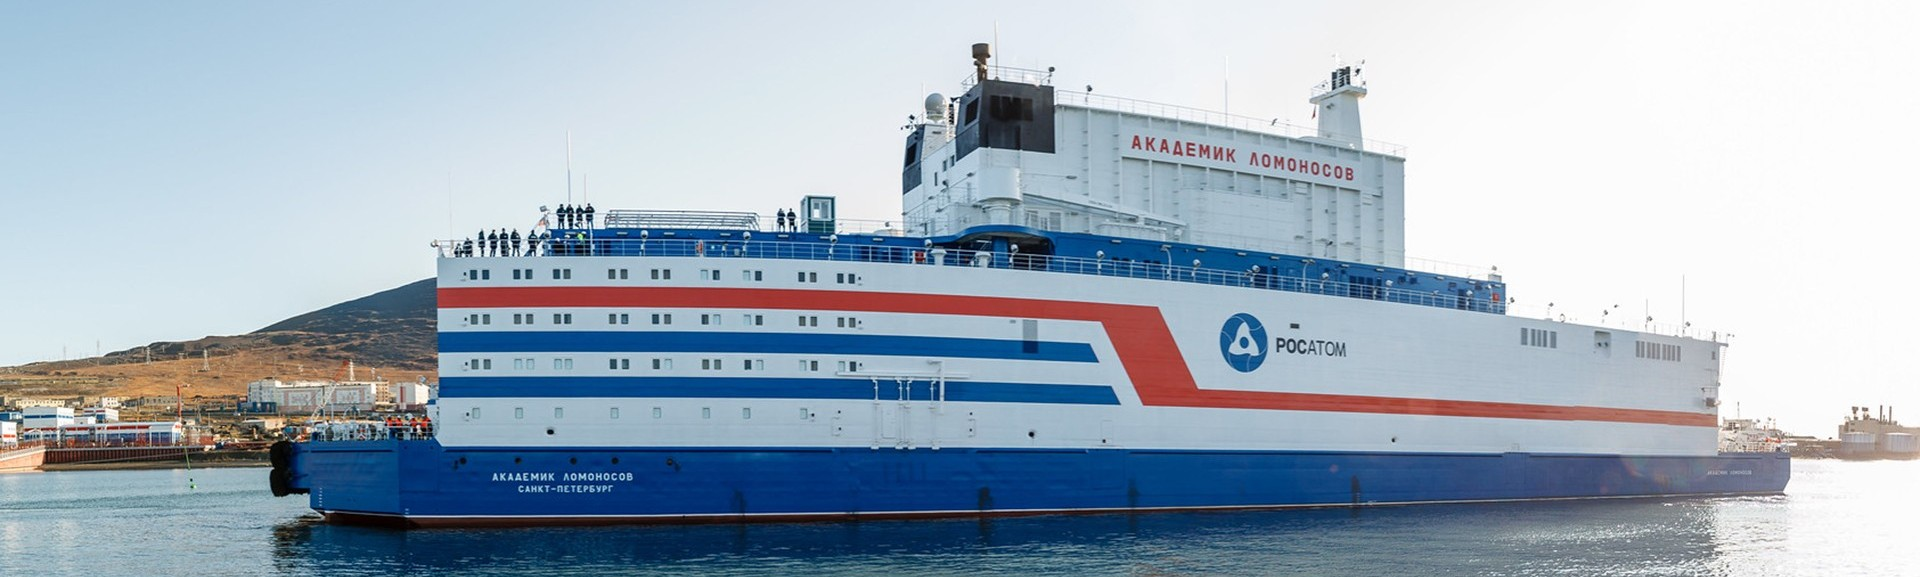
\includegraphics[width=0.8\textwidth]{content/figures/akademik_lomonosov.jpg}
    \caption{La central nuclear flotante Akademik Lomonosov (\cite{nuclear_españa}).}
    \label{fig:akademik_lomonosov}
\end{figure}

\item \underline{\acrshortpl{smr} refrigerados por gas de alta temperatura (del inglés, \acrshort{htgr}):} Reactores de \acrshort{genIV} que proporcionan calor a elevada temperatura (superior a 750°C) y que pueden ser utilizados para generar electricidad de forma más eficiente y con una variedad de aplicaciones industriales. Dentro de esta categoría, hay múltiples diseños en desarrollo y alguno en operación, como el \textbf{HTR-PM de China, el primer \acrshort{htgr} en operación del mundo}. Con un reactor de lecho de bolas\footnote{Reactor de muy alta temperatura moderado con grafito y refrigerado por gas, cuyos elementos de combustible son esféricos (denominados ``bolas'') y contienen miles de partículas \acrshort{triso}. Estos combustibles tri-isotrópicos constan de carburo de uranio revestido con varias capas de carbón pirolítico y dióxido de silicio para retener los productos de fisión a altas temperaturas.}, una potencia eléctrica de 210 MWe y una potencia térmica de 500 MWt, se conectó a la red en diciembre de 2021 y comenzó a operar comercialmente a plena potencia en diciembre de 2023, con el objetivo de reemplazar las centrales de carbón presentes en el interior de China. También se incluyen en este grupo tres reactores de prueba \acrshort{htgr}, dos de los cuales han estado en operación durante más de veinte años para realizar pruebas en Japón y China.

\item \underline{\acrshortpl{smr} refrigerados por metal líquido de espectro rápido de neutrones:} Los metales líquidos que utilizan como regrigerantes incluyen sodio, plomo puro y eutéctico de plomo-bismuto. Hay grandes avances en el desarrollo y despliegue de esta tecnología de \acrshortpl{smr}. Prueba de ello es el BREST-OD-300, un reactor de neutrones rápidos refrigerado por plomo que se está construyendo en Seversk (Rusia) y se planea su puesta en marcha en 2026. Se trata de un proyecto prototipo para futuros diseños que empleen un ciclo combustible nuclear cerrado, en el cual pueda reutilizarse el combustible gastado mediante la separación del uranio, plutonio y actínidos minoritarios (Np, Am y Cm), para ser transmutados en estos reactores rápidos (\cite{apuntes_centrales}).

\item \underline{\acrshortpl{smr} de sales fundidas (del inglés, \acrshortpl{msr}):} Reactores de \acrshort{genIV} alimentados y refrigerados por sales fundidas, propiedad que les confiere múltiples ventajas, incluida una seguridad mejorada debido a la propiedades de las sales, un sistema de refrirefrigeración de fase única a baja presión que elimina la necesidad de un gran contenedor, un sistema de alta temperatura con gran eficiencia y un ciclo de combustible flexible. Se están llevando a cabo actividades preliminares de licenciamiento con varios de estos diseños con reguladores de Canadá, Dinamarca, Países Bajos, Reino Unido y los Estados Unidos.

\item \underline{Microreactores modulares (del inglés, \acrshortpl{mmr}):} Diseños de \textbf{menos de 10 MWe de potencia}, con capacidad de opearción semi-autónoma y con una mejor transportabilidad que los \acrshortpl{smr} más grandes. Existen varios diseños punteros tecnológicamente ---incluidos de \acrshort{genIV}---, en los que el reactor utiliza diversos refrigerantes en cada caso: agua ligera, helio, sales fundidas o metal líquido. Los \acrshortpl{mmr} son especialmente adecuados para operar fuera de la red en ubicaciones remotas, en situaciones de necesidad de abastecimiento de emergencia en hospitales o comunidades afectadas por desastres naturales, para desalinizar agua del mar, etc. Estos microrreactores se encuentran en las primeras fases de desarrollo y, en las aplicaciones concretas anteriormente expuestas, se espera que sean muy competitivos frente a las fuentes de electricidad previamente utilizadas.

\begin{figure}[h]
    \centering
    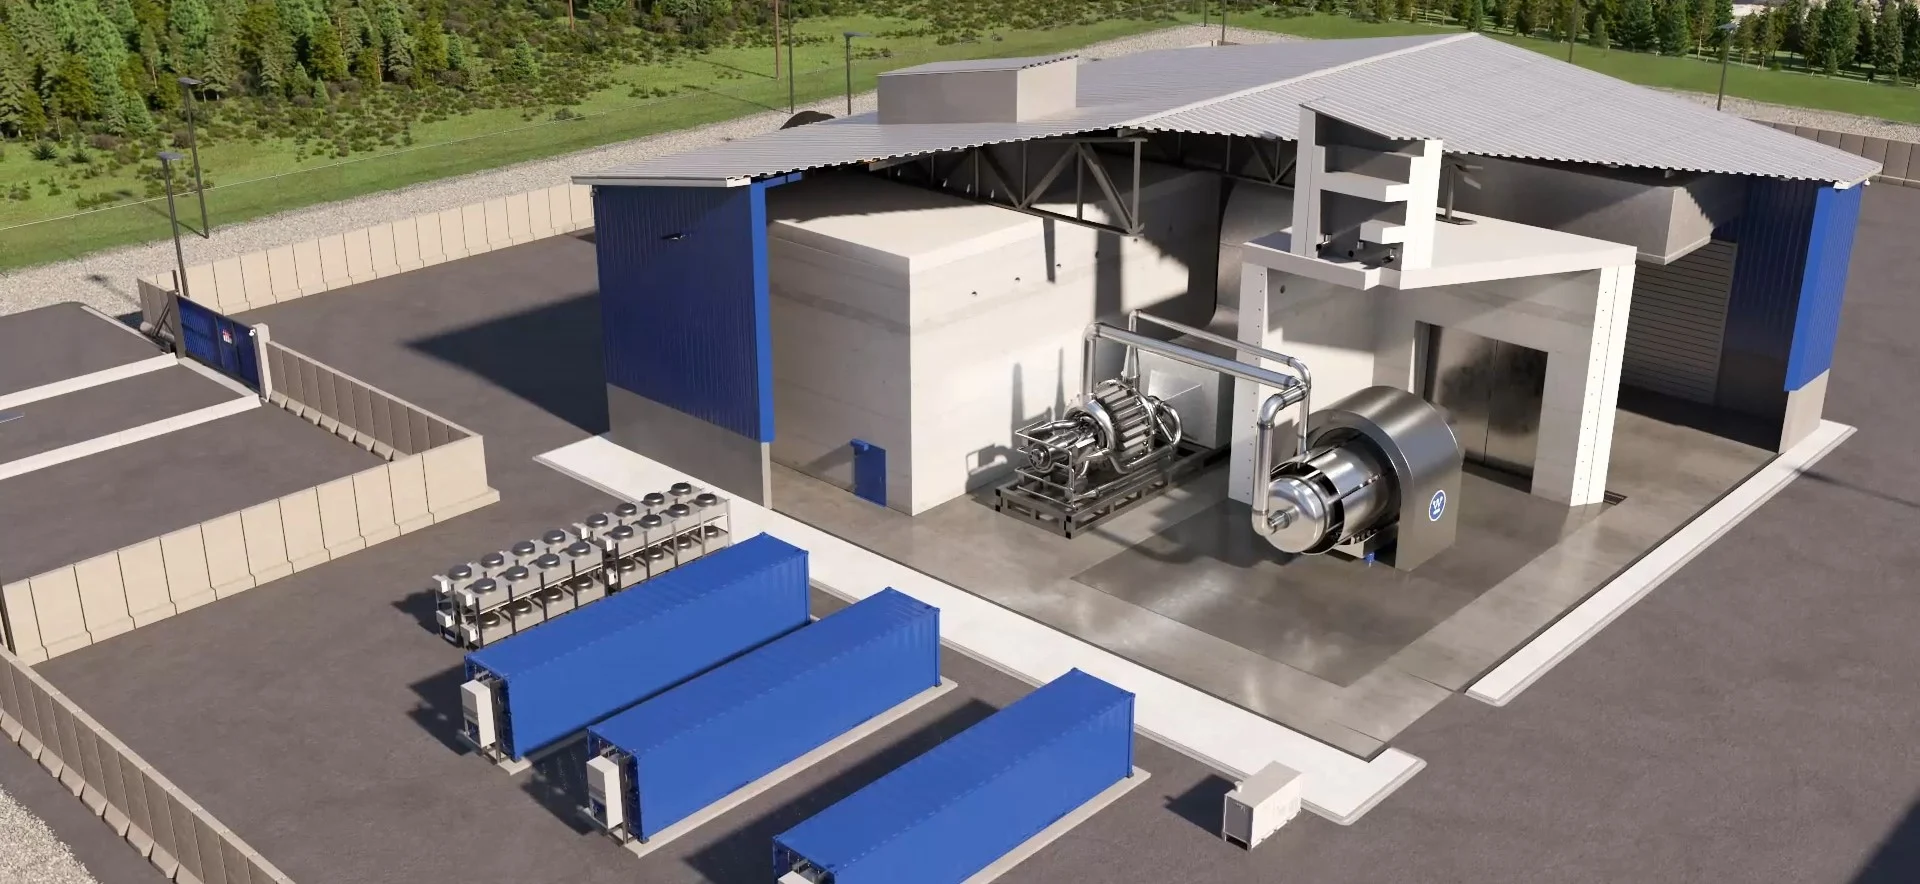
\includegraphics[width=0.6\textwidth]{content/figures/evinci.jpg}
    \caption{Render del \emph{eVinci$^{TM}$ Microreactor} de Westinghouse, con una potencia de 5 MWe y 13 MWt (\cite{evinci}).}
    \label{fig:evinci}
\end{figure}

\end{enumerate}

\subsection{Características generales}

Los diseños de \acrshortpl{smr} están progresando gradualmente, partiendo del objetivo de integrar sistemas para conseguir modulizar los reactores al mismo tiempo que se introducen mejoras significativas para el funcionamiento eficaz y seguro de los mismos. De esta manera, se están desarrollando prototipos con muy buenas prestaciones en lo que a seguridad, flexibilidad, costes, gestión de residuos y variedad de aplicaciones se refiere.

\subsubsection{Seguridad}

Debido a la experiencia de más de 60 años de operación de las centrales nucleares, se han llevado a cabo gradualmente grandes mejoras de seguridad y control de las mismas. Los reactores nucleares avanzados que se están desarrollando en los últimos años, incluidos los \acrshortpl{smr}, incorporan estos avances tecnológicos. Entre las múltiples mejoras incorporadas, cabe destacar el empleo de innovadores \textbf{sistemas de seguridad pasiva}. Los sistemas pasivos son aquellos que no requieren de la acción de un operador o de realimentación electrónica para funcionar, sino que su actuación se asegura por principios físicos independientes de energía externa. Son, por tanto, especialmente útiles en casos de emergencia en los que, aunque se perdiera el suministro eléctrico de la central, los sistemas de seguridad deberían funcionar sin ningún problema (\cite{glosario_seguridad_oiea}). Algunos ejemplos de este tipo de sistemas son los recombinadores autocatalíticos pasivos\footnote{Eliminan los posibles gases combustibles generados dentro de la contención en accidentes severos mediante la recombinación o combustión de una manera gradual, minimizando así el riesgo de una explosión de hidrógeno.}, el \acrfull{svfc}\footnote{Posibilita la despresurización controlada del Edificio de Contención en caso de fusión del núcleo y la reducción de la cantidad de material radiactivo que podría ser liberado al exterior.} o el sistema de sellado pasivo de las bombas del circuito primario\footnote{Permite reducir significativamente o, incluso, eliminar la fuga de refrigerante a través de los sellos sin requerir operación manual. Se activan por temperatura y bloquean automáticamente
el paso de agua.}. Todas estas nuevas implementaciones ya forman parte de los sistemas de seguridad de los reactores avanzados.

En el caso de los \acrshortpl{smr}, su diseño integral incorpora todos los componentes del sistema de suministro de vapor nuclear (del inglés, \acrshort{nsss}) en un solo recipiente, aumentando así la capacidad calorífica e inercia térmica, la seguridad inherente, así como una operación y mantenimiento más simples.

La menor potencia de salida y mayor relación superficie-volumen de núcleos más pequeños aumenta la eficiencia de los sistemas de SEGURIDAD pasiva. Los sistemas de refrigeración pasivos permiten diseños más simplificados y una operación y mantenimiento optimizados.

\subsubsection{Flexibilidad y modularidad}

El tamaño más pequeño de los diseños SMR permite la adopción de más ambiciosos esquemas de MODULARIZACIÓN, así como nuevas técnicas de fabricación. Los distintos componentes se pueden fabricar, transportar e izar con mucha mayor facilidad que en los reactores convencionales.

Los SMR incorporan FLEXIBILIDAD con modos de seguimiento de carga mejorados incorporados en el diseño, así como a través de la optimización de operación de unidades de múltiples módulos. La flexibilidad también permite la producción combinada de calor y electricidad.

\subsubsection{Reducción de costes y competitividad}
ECONOMÍA
Los SMR están basados en la economía de producción en serie con varios factores clave de costes: simplificación del diseño, estandarización y modularización, maximizando al mismo tiempo la fabricación en fábrica y minimizando la construcción en el destino final.

La mayor integración del diseño ofrece nuevas oportunidades para la simplificación de los sistemas SMR. Algunos componentes activos, por ejemplo, bombas de refrigeración del reactor y sus sistemas auxiliares ya no son necesarios en los nuevos diseños, abaratando los costes.

La posibilidad de construir SMR bajo tierra y el uso de sistemas de aislamiento sísmico reduciría la necesidad de adaptar los diseños a la sismología local. La modularización simplifica la construcción y también baja los costes, como ocurre en la construcción naval y aeronáutica.

La construcción en fábrica también puede presentar beneficios adicionales, en particular en términos de aplicación de técnicas de fabricación avanzadas, como soldadura láser, lo que permitirá reducir costes y eliminar costosas inspecciones en servicio.

Los diseños SMR podrían presentar una opción de inversión atractiva en comparación con grandes LWR: menor desembolso de capital, menor riesgo, recuperación más rápida de la inversión, menor coste con la fabricación en serie, mayor flexibilidad y servicios auxiliares a la red.

\subsubsection{Mejora en la gestión de residuos}
Una MENOR CANTIDAD DE COMBUSTIBLE requiere menos protección y reduce la dosis radiactiva a trabajadores, el riesgo de accidente y las zonas de planificación de emergencia. Algunos SMR pueden estar ubicados más cerca de donde se necesita energía.

COMBUSTIBLE
Se espera que los LWR-SMR desarrollen ciclos de combustible compatibles con los actuales, con enriquecimientos por debajo del 5\%. No se descarta que los SMR utilicen óxido mixto de uranio (MOX). Se esperan ciclos de operación más largos que en los LWR existentes.

Los microrreactores y SMR de IV Generación se espera que tengan periodos de operación entre recargas de combustible de hasta 20 años. Los reactores que funcionan con combustible triestructural-isotrópico (TRISO) o con sales fundidas pueden recargar sin dejar de funcionar.

Varios diseños están considerando el uso de combustible de uranio poco enriquecido (entre el 5 y el 19,75\%) de alto rendimiento: HALEU.

Tabla con el ciclo de combustible de cada uno de los grupos de SMR.
\subsubsection{Diversdidad de aplicaciones}

APLICACIONES
Los SMR podrían apoyar la descarbonización de otros sectores energéticos, como la calefacción urbana, que requiere temperaturas de salida entre 80 y 200°C. Arabia Saudí también tiene interés en los SMR para cumplir sus necesidades de desalación del agua del mar.

Las temperaturas más altas proporcionadas por algunos SMR de IV Generación (450-850°C) puede servir para descarbonizar sectores industriales difíciles de sustituir hasta ahora, como refinado de petróleo, reformado con vapor para gas natural y producción de hidrógeno termoquímico.

Los SMR tienen características inherentes de seguimiento de carga que los hacen capaces de realizar una operación flexible en redes con una gran penetración de energías renovables variables, como eólica y solar fotovoltaica.

Los SMR se pueden implementar en áreas remotas y aisladas que no están conectadas a la red, en regiones con pequeñas redes eléctricas o en regiones con sitios adecuados limitados para grandes instalaciones nucleares.

En la Hoja de ruta de los SMR canadienses de 2018 se identificaron varias comunidades remotas fuera de la red e instalaciones mineras, donde los SMR podrían ser rentables como reemplazo de generadores diésel.


\subsection{Tecnologías en fase avanzada de diseño}

En todo el mundo existen más de 80 diseños y conceptos de SMR. La mayoría de ellos están en diversas etapas de desarrollo y de algunos se afirma que podrán desplegarse a corto plazo.

\begin{figure}[h]
    \centering
    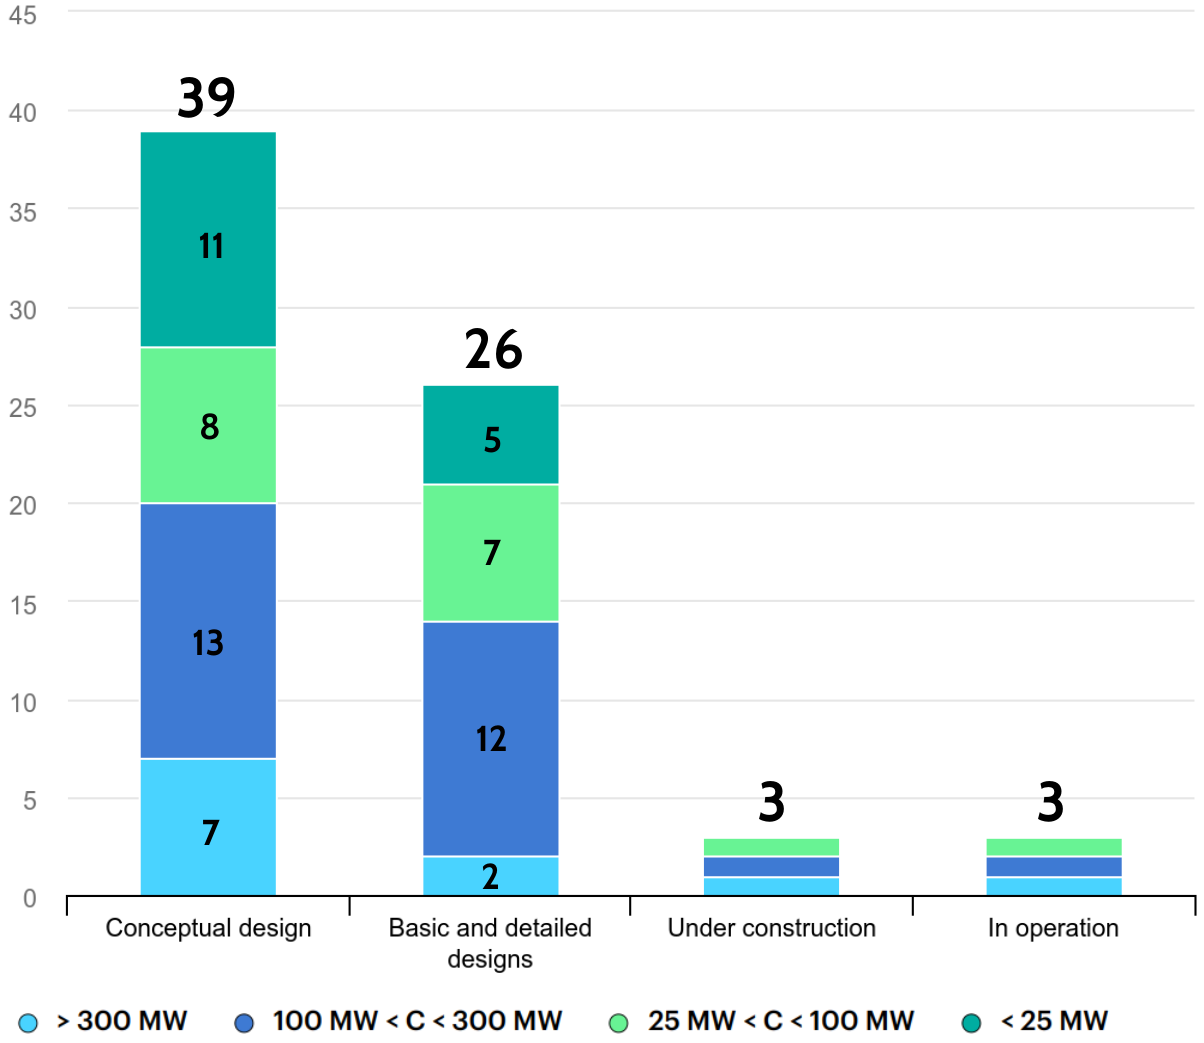
\includegraphics[width=0.7\textwidth]{content/figures/global_smr_projects.png}
    \caption{Número de proyectos de \acrshortpl{smr} en el mundo por estados de desarrollo (\cite{iea_global_smr_projects}).}
    \label{fig:global_smr_projects}
\end{figure}

Actualmente existen cuatro SMR en etapas avanzadas de construcción en Argentina, China y Rusia, y varios países en el ámbito de la energía nuclear y en fase de incorporación están llevando a cabo actividades de investigación y desarrollo de SMR.

\subsection{Tecnologías en operación}

\subsection{Reactor AP300}